\TUsection{Quantitative Evaluation of Iterative Symbolic Executions}

The process carried out by the iterative reduce strategy resembles to a loop unwinding technique, where an iterative behavior is taken out of a loop and executed sequentially without the need of accumulators or counters. This approach is often used to improve execution speed of a program by getting rid of all the control flow instructions inherent to loop statements. However, regarding \textit{JPF-SymSpark} and several other program analysis techniques, loop unwinding is used to bound the execution of potentially infinite loop instructions, hence allowing the evaluation of the program under test.

\textit{JPF-SymSpark} allows the user to specify the number of iterations of an aggregated function that will be symbolically executed. This enables the module to bound the execution of the iterative behavior and carry out the analysis by correctly chaining the outcome of previous iterations. However, the number of path conditions grow exponentially with the number of conditional statements found. This means that if the aggregate function being analyzed has a conditional statement, then it is most likely that a path explosion will occur.

This evaluation focuses on the behavior of the iterative reduce strategy and it aims to identify the major aspects that pose performance losses. It illustrates how an increment in the number of iterations to be considered in the analysis has a direct impact in the number and size of path conditions, as well as in the performance of the constraint solvers. Moreover, it serves as an example to identify path explosion in symbolic executions.

\TUsubsection{Setup}

Four scenarios were considered for the experiments:

\begin{itemize}
	\item \textbf{Iterative Reduce with Non Cumulative Condition (IRNC)}: The program under test contains a single \textit{reduce} action with a conditional instruction defined only over a non cumulative symbolic variable.
	\item \textbf{Iterative Reduce with Cumulative Condition (IRC)}: Also a single \textit{reduce} action but this time the conditional instruction is defined over the cumulative symbolic variable.
	\item \textbf{Iterative Map and Reduce with Non Cumulative Condition (IMRNC)}: This scenario is similar to the first one with the difference that the \textit{reduce} action is preceded by a \textit{map} transformation with a single conditional statement over its symbolical variable.
	\item \textbf{Iterative Map and Reduce with Cumulative Condition (IMRC)}: Same as the previous scenario except that the \textit{reduce} action has a conditional instruction defined over its cumulative symbolic variable.
\end{itemize}

The first two scenarios aim to determine what kind of performance effects generate from solving constraints based on cumulative and non cumulative constraints. The last two scenarios are used to measure the relevance of previous transformations that manipulate the symbolic variable and also introduce a condition to the path before the \texttt{reduce} action. All the scenarios were implemented as trivial Spark programs processing only integer values. Furthermore, the conditional statements between operations were defined in a way that unsatisfiable path conditions would be generated eventually.

Each scenario was executed for 2, 3, 5, 8 and 13 iterations respectively, repeating each case ten times and taking the average of the execution time as the result. This range follows a Fibonacci sequence and was chosen to space out the iterations enough to make any trend distinguishable. Additionally, for each case, the number of satisfiable and unsatisfiable path conditions was registered. The experiments were carried out in a laptop computer with an Intel Core-i7-6500U processor at 2.50GHz and assigning 1GB of memory to the JVM executing the analysis. \jpf{} was triggered using the command line instead of the Eclipse JPF plugin in order to avoid wasting memory in processes inherent to the Eclipse IDE.

\TUsubsection{Results and Discussion}

The results of the experiments are summarized in table~\ref{tab:evaluation:quantitative-time} for the executions times, and in table~\ref{tab:evaluation:quantitative-path-conditions} for the number of satisfiable and unsatisfiable path condition for each scenario.

\textbf{Execution times}

All the scenarios have a similar performance up until three symbolic iterations. However, the performance of some scenarios start to diverge after five iterations. The starkest difference is displayed by the \textit{IRC} scenario, where the execution times increase several orders of magnitude in comparison to the other scenarios. In particular, the \textit{IRC} scenario could not be executed for 13 iterations or more, resulting in executions that lasted several hours and culminating eventually in \textit{OutOfMemory} exceptions.

The rest of the scenarios have a steady increase in their measurements until they reach 13 symbolic iterations, where the execution times start to grow exponentially. From the remaining three scenarios, the \textit{IMRC} scenario displays the worst performance, taking almost three minutes to execute 13 symbolic executions. Figure~\ref{fig:evaluation:quantitative} presents a plot of the execution times in a logarithmic scale that better depicts the disparity between some of the scenarios.

\begin{table}[t]
	\centering
	\small
	\begin{tabular*}{0.9\textwidth}{@{\extracolsep{\fill}} lccccc}
		\hline
		Iterations & 2 & 3 & 5 & 8 & 13 \\
		\hline\hline
		IRNC  & 0.680 & 0.705 & 0.855  & 1.344   & 5.489   \\
		IRC   & 0.589 & 0.625 & 15.616 & 568.004 & N/A      \\
		IMRNC & 0.669 & 0.710 & 0.981  & 2.621   & 21.662  \\
		IMRC  & 0.681 & 0.728 & 1.144  & 2.585    & 177.579 \\
		\hline	
	\end{tabular*}	
	\caption[Average Execution Times]{Average execution time in seconds for each scenario under the different number of executed iterations.}
	\label{tab:evaluation:quantitative-time}
\end{table}

\begin{figure}
	\centering	
	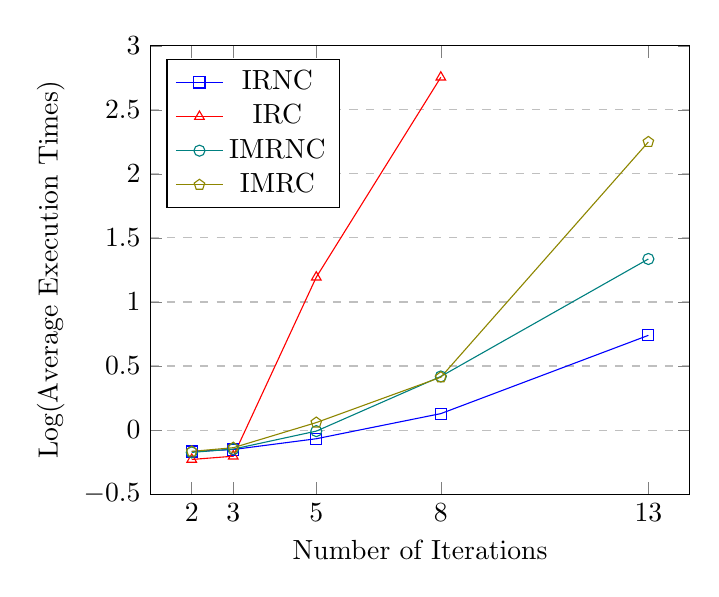
\begin{tikzpicture}
		\begin{axis}[
%			title={Average Execution Times in Log10},
			xlabel={Number of Iterations},
			ylabel={Log(Average Execution Times)},
			xmin=1, xmax=14,
			ymin=-0.5, ymax=3,
			xtick={2,3,5,8,13},
			ytick={-0.5,0,0.5,1,1.5,2,2.5,3},
			legend pos=north west,
			ymajorgrids=true,
			grid style=dashed,
		]
			
			\addplot[
			color=blue,
			mark=square,
			]
			coordinates {
				(2,-0.1673633724)(3,-0.151810883)(5,-0.0676277179)(8,0.1284638911)(13,0.739524878)
			};
	
			\addplot[
			color=red,
			mark=triangle,
			]
			coordinates {
				(2,-0.2294425251)(3,-0.2040505011)(5,1.1935725814)(8,2.7543517764)
			};
			
			\addplot[
			color=teal,
			mark=o,
			]
			coordinates {
				(2,-0.1741197011)(3,-0.148619332)(5,-0.0081539464)(8,0.4185829941)(13,1.3357165949)
			};
			
			\addplot[
			color=olive,
			mark=pentagon,
			]
			coordinates {
				(2,-0.1663430031)(3,-0.1376300629)(5,0.058615797)(8,0.4124605474)(13,2.2493920951)
			};
	
			\legend{IRNC, IRC, IMRNC, IMRC}
		\end{axis}
	\end{tikzpicture}
	\caption[Average Execution Times in Logarithmic Scale]{Average execution times in logarithmic scale. The disparity between the scenarios is easily perceived using a logarithmic scale while still preserving the notion of exponential growth.}
	\label{fig:evaluation:quantitative}
\end{figure}


\textbf{Number of path conditions}

As expected, the total number of path conditions grows exponentially over the number of iterations executed. The scenarios having a \textit{map} transformation before the iterative action have double the total amount of path conditions than their counterparts without the transformation. This is consistent to the exponential growth of the number of path conditions given that the transformation only introduced an additional branching statement.

Nevertheless, the number of non satisfiable path conditions varies strongly depending on the scenario being studied. In the case of the \textit{IRNC} scenario, all path conditions are satisfiable, while for the \textit{IRC} scenario, only a few in the case of 8 iterations are not satisfiable; most of these resulting from timeouts of the constraint solvers. On the contrary, the \textit{IMRNC} and \textit{IMRC} scenarios present high rates of unsatisfiable path conditions throughout the different number of iterations, ranging from 30\% to 50\% for the former and from 45\% to 90\% for the latter.

\textbf{Discussion}

The results obtained in these experiments highlight some key features on the behavior of symbolic execution of aggregate functions. First, the performance of the framework is considerably better when the conditional statements defined in the aggregate function only affect the non-cumulative symbolic variable in the operation. This comes as a consequence of the kind of constraints generated in such cases. In the case of non-cumulative conditions, the constraints are defined over single independent symbolic variables that are joined in a conjunction on each iteration, while in the case of cumulative conditions, after each iteration, the constraints include more symbolic variables related with each other. Constraint solvers perform better when the constraints are defined over independent symbolic variables, which explains the behavior of the \textit{IRC} scenario and the difference between the cumulative and non-cumulative scenarios in general.

Another aspect is the difference between the \textit{IRC} and \textit{IMRC} scenarios. After five iterations, the behavior of these two scenarios diverges strongly, having the \textit{IRC} scenario performing exponentially worse and even reaching the point of not being able to finish its execution, while the \textit{IMRC} scenario is still capable to finish the execution within a reasonable amount of time. The reason for this relies in the number of unsatisfiable path conditions in the \textit{IMRC} scenario because, although this scenario has more path conditions than the \textit{IMC} scenario, a large number of them are unsatisfiable, allowing the constraint solver to conclude faster. This result indicates that having more path conditions does not necessarily translates into worse performance; it depends on how complex the path conditions are and how many of them are actually satisfiable.

The performance of the constraint solver as well as the complexity of the path conditions are the major factors that affect the overall performance of iterative symbolic executions in \textit{JPF-SymSpark}. Moreover, the construction of aggregate functions with conditional statements has to be properly evaluated in terms of the congruency of the operation. Conditions applied to a cumulative value can break the associativity requirement of reducer functions, leading to invalid, non-parallelizable Spark programs.

\begin{table}[t]
	\centering
	\small
	\begin{tabular*}{0.9\textwidth}{@{\extracolsep{\fill}} lcc|cc|cc|cc|cc}
		\hline
		Iterations & \multicolumn{2}{c}{2} & \multicolumn{2}{c}{3} & \multicolumn{2}{c}{5} & \multicolumn{2}{c}{8} & \multicolumn{2}{c}{13} \\
		&  s & u & s & u & s & u & s & u & s & u \\		
		\hline\hline
		IRNC   & 6 & 0 & 14 & 0  & 62 & 0  & 510 & 0   & 16382 & 0     \\
		IRC    & 6 & 0 & 14 & 0  & 62 & 0  & 454 & 56  & n/a & n/a     \\
		IMRNC  & 8 & 4 & 17 & 11 & 67 & 57 & 518 & 512 & 16395 & 16369 \\
		IMRC   & 7 & 5 & 12 & 16 & 25 & 99 & 57  & 963 & 573   & 32191 \\
		\hline	
	\end{tabular*}
	\caption[Number of Satisfiable and Unsatisfiable Path Conditions]{Number of satisfiable and unsatisfiable path conditions for each scenario under the different number of executed iterations. As a reference, the letter ``s'' stands for satisfiable while the letter ``u'' stands for unsatisfiable.}
	\label{tab:evaluation:quantitative-path-conditions}
\end{table} 